\appendix

\section{Appendix A: Transfer Entropy and Its Estimation from Data}

Let $\{X_{t}\}$ and $\{ Y_{t}\}$ be two strong-sense stationary stochastic processes\footnote{Recall that a stochastic process is strong-sense stationary if the joint distribution for the process evaluated at finitely many time points is invariant to an overall timeshift~\cite{grimmett2001probability}.}. In our work, these would correspond to the activities, $X_{t}(u)$ and $X_{t}(v),$ of two users $u$ and $v$. We use the notation $X_{t-k}^{t}$ to denote the values of the stochastic process from time $t-k$ to time $t$, $X_{t-k}^{t} = (X_{t-k}, X_{t-(k-1)}, \ldots, X_{t - 1}, X_{t})$. The lag-$k$ transfer entropy~\cite{schreiber2000measuring} of $Y$ on $X$ is defined as 
\begin{align}
	\text{TE}_{Y \to X}^{(k)} &= H\left[X_{t} | X_{t-k}^{t-1}\right] - H\left[X_{t} | X_{t-k}^{t-1}, Y_{t-k}^{t-1}\right], \label{Eqn-TE}
\end{align}
where
\begin{align}
	H\left[X_{t} | X_{t-k}^{t-1}\right] = - E\left[ \log_{2} p(X_{t} | X_{t-k}^{t-1}) \right]
\end{align}
and 
\begin{align}
	H\left[X_{t} | X_{t-k}^{t-1}, Y_{t-k}^{t-1}\right] = - E\left[ \log_{2} p(X_{t} | X_{t-k}^{t-1}, Y_{t-k}^{t-1}) \right]
\end{align}
are the usual conditional entropies over the conditional (predictive) distributions $p(x_{t} | x_{t-k}^{t-1})$ and $p(x_{t} | x_{t-k}^{t-1}, y_{t-k}^{t-1})$. This formulation was originally developed in~\cite{schreiber2000measuring}, where transfer entropy was proposed as an information theoretic measure of \emph{directed} information flow. Formally, recalling that $H\left[X_{t} | X_{t-k}^{t-1}\right]$ is the uncertainty in $X_{t}$ given its values at the previous $k$ time points, and that $H\left[X_{t} | X_{t-k}^{t-1}, Y_{t-k}^{t-1}\right]$ is the uncertainty in $X_{t}$ given the joint process $\{(X_{t}, Y_{t})\}$ at the previous $k$ time points, transfer entropy measures the reduction in uncertainty of $X_{t}$ by including information about $Y_{t-k}^{t-1},$ controlling for the information in $X_{t - k}^{t-1}$. By the `conditioning reduces entropy' result~\cite{cover2012elements}
\begin{align}
	H[X | Y, Z] \leq H[X | Y],
\end{align}
we can see that transfer entropy is always non-negative, and is zero precisely when $H\left[X_{t} | X_{t-k}^{t-1}\right] = H\left[X_{t} | X_{t-k}^{t-1}, Y_{t-k}^{t-1}\right]$, in which case knowing the past $k$ lags of $Y_{t}$ does not reduce the uncertainty in $X_{t}$. If the transfer entropy is positive, then $\{ Y_{t}\}$ is considered causal for $\{ X_{t}\}$ in the Granger sense~\cite{granger1963economic}.

In estimating the transfer entropy from finite data, we will assume that the process $\{(X_{t}, Y_{t})\}$ is jointly stationary, which gives us that
\begin{align}
	p(x_{t} | x_{t-k}^{t-1}) = p(x_{k+1} | x_{1}^{k})
\end{align}
and
\begin{align}
	p(x_{t} | x_{t-k}^{t-1}, y_{t-k}^{t-1}) = p(x_{k+1} | x_{1}^{k}, y_{1}^{k})
\end{align}
for all $t$. That is, the predictive distribution only depends on the past, not on when the past is observed. Given this assumption, we compute estimators for $p(x_{k+1} | x_{1}^{k})$ and $p(x_{k+1} | x_{1}^{k}, y_{1}^{k})$ by `counting': for each possible marginal and joint past $x_{1}^{k}$ and $(x_{1}^{k}, y_{1}^{k})$, we count the number of times a future of type $x_{k+1}$ occurs, and normalize to obtain the appropriate estimators of the one-step-ahead predictive distributions. Call these estimators $\hat{p}(x_{k+1} | x_{1}^{k})$ and $\hat{p}(x_{k+1} | x_{1}^{k}, y_{1}^{k})$. Then the plug-in estimator for the transfer entropy is
\begin{align}
	\widehat{\text{TE}}_{Y \to X}^{(k)} &= \hat{H}\left[X_{t} | X_{t-k}^{t-1}\right] - \hat{H}\left[X_{t} | X_{t-k}^{t-1}, Y_{t-k}^{t-1}\right]
\end{align}
where we use the plug-in estimators $\hat{H}\left[X_{t} | X_{t-k}^{t-1}\right]$ and $\hat{H}\left[X_{t} | X_{t-k}^{t-1}, Y_{t-k}^{t-1}\right]$ for the entropies. It is well known that the plug-in estimator for entropy is biased~\cite{paninski2003estimation}. To account for this bias, we use the Miller-Madow adjustment to the plug-in estimator~\cite{miller1955note}. For a random variable $X$ taking on finitely many values from an alphabet $\mathcal{X}$, the Miller-Madow estimator is
	\begin{align}
		\tilde{H}[X] = \hat{H}[X] + \frac{|\hat{\mathcal{X}}| - 1}{2 n}
	\end{align}
	where $|\mathcal{\hat{X}}|$ is the number of observed symbols from the alphabet $\mathcal{X}$ and $n$ was the number of samples used to estimate $\hat{H}[X].$ The definition of transfer entropy~(\ref{Eqn-TE}) can be rewritten in terms of joint entropies as
	\begin{align}
		TE_{Y \to X}^{(k)} &= H[X_t | X_{t-k}^{t-1}] - H[X_t | X_{t-k}^{t-1},Y_{t-k}^{t-1}] \\ 
		&= H[X_t,X_{t-k}^{t-1}]-H[X_{t-k}^{t-1}]-H[X_t,X_{t-k}^{t-1},Y_{t-k}^{t-1}]+H[X_{t-k}^{t-1},Y_{t-k}^{t-1}],
	\end{align}
	We then apply the Miller-Madow adjustment individually to each of the entropy terms. For example, for the first term, we have
	\begin{align}
		\tilde{H}[X_{t}, X_{t - k}^{t-1}] = \tilde{H}[X_{t - k}^{t}] = \hat{H}[X_{t-k}^{t}] + \frac{|\widehat{\mathcal{X}^{k+1}}| - 1}{2n},
	\end{align}
	where $|\widehat{\mathcal{X}^{k+1}}|$ is the number of $(k + 1)$-tuples we actually observe (of the $2^{k + 1}$ possible tuples). Doing this for each term, the overall Miller-Madow estimator for the transfer entropy is
	\begin{align}
		\widetilde{TE}_{Y \to X}^{(k)} &= \tilde{H}[X_t | X_{t-k}^{t-1}] - \tilde{H}[X_t | X_{t-k}^{t-1},Y_{t-k}^{t-1}] \\ 
		&= \tilde{H}[X_t,X_{t-k}^{t-1}]-\tilde{H}[X_{t-k}^{t-1}]-\tilde{H}[X_t,X_{t-k}^{t-1},Y_{t-k}^{t-1}]+\tilde{H}[X_{t-k}^{t-1},Y_{t-k}^{t-1}].
	\end{align}
	One possible problem with this estimator is that it can result in \emph{negative} estimates of entropies. That usually occurs when $\hat{H}$ is very small. In these cases, we truncate set the estimator to zero.

\section{Appendix B: Comparing Edges Across Different Community Types}

\begin{figure}[!h]
	\centering
	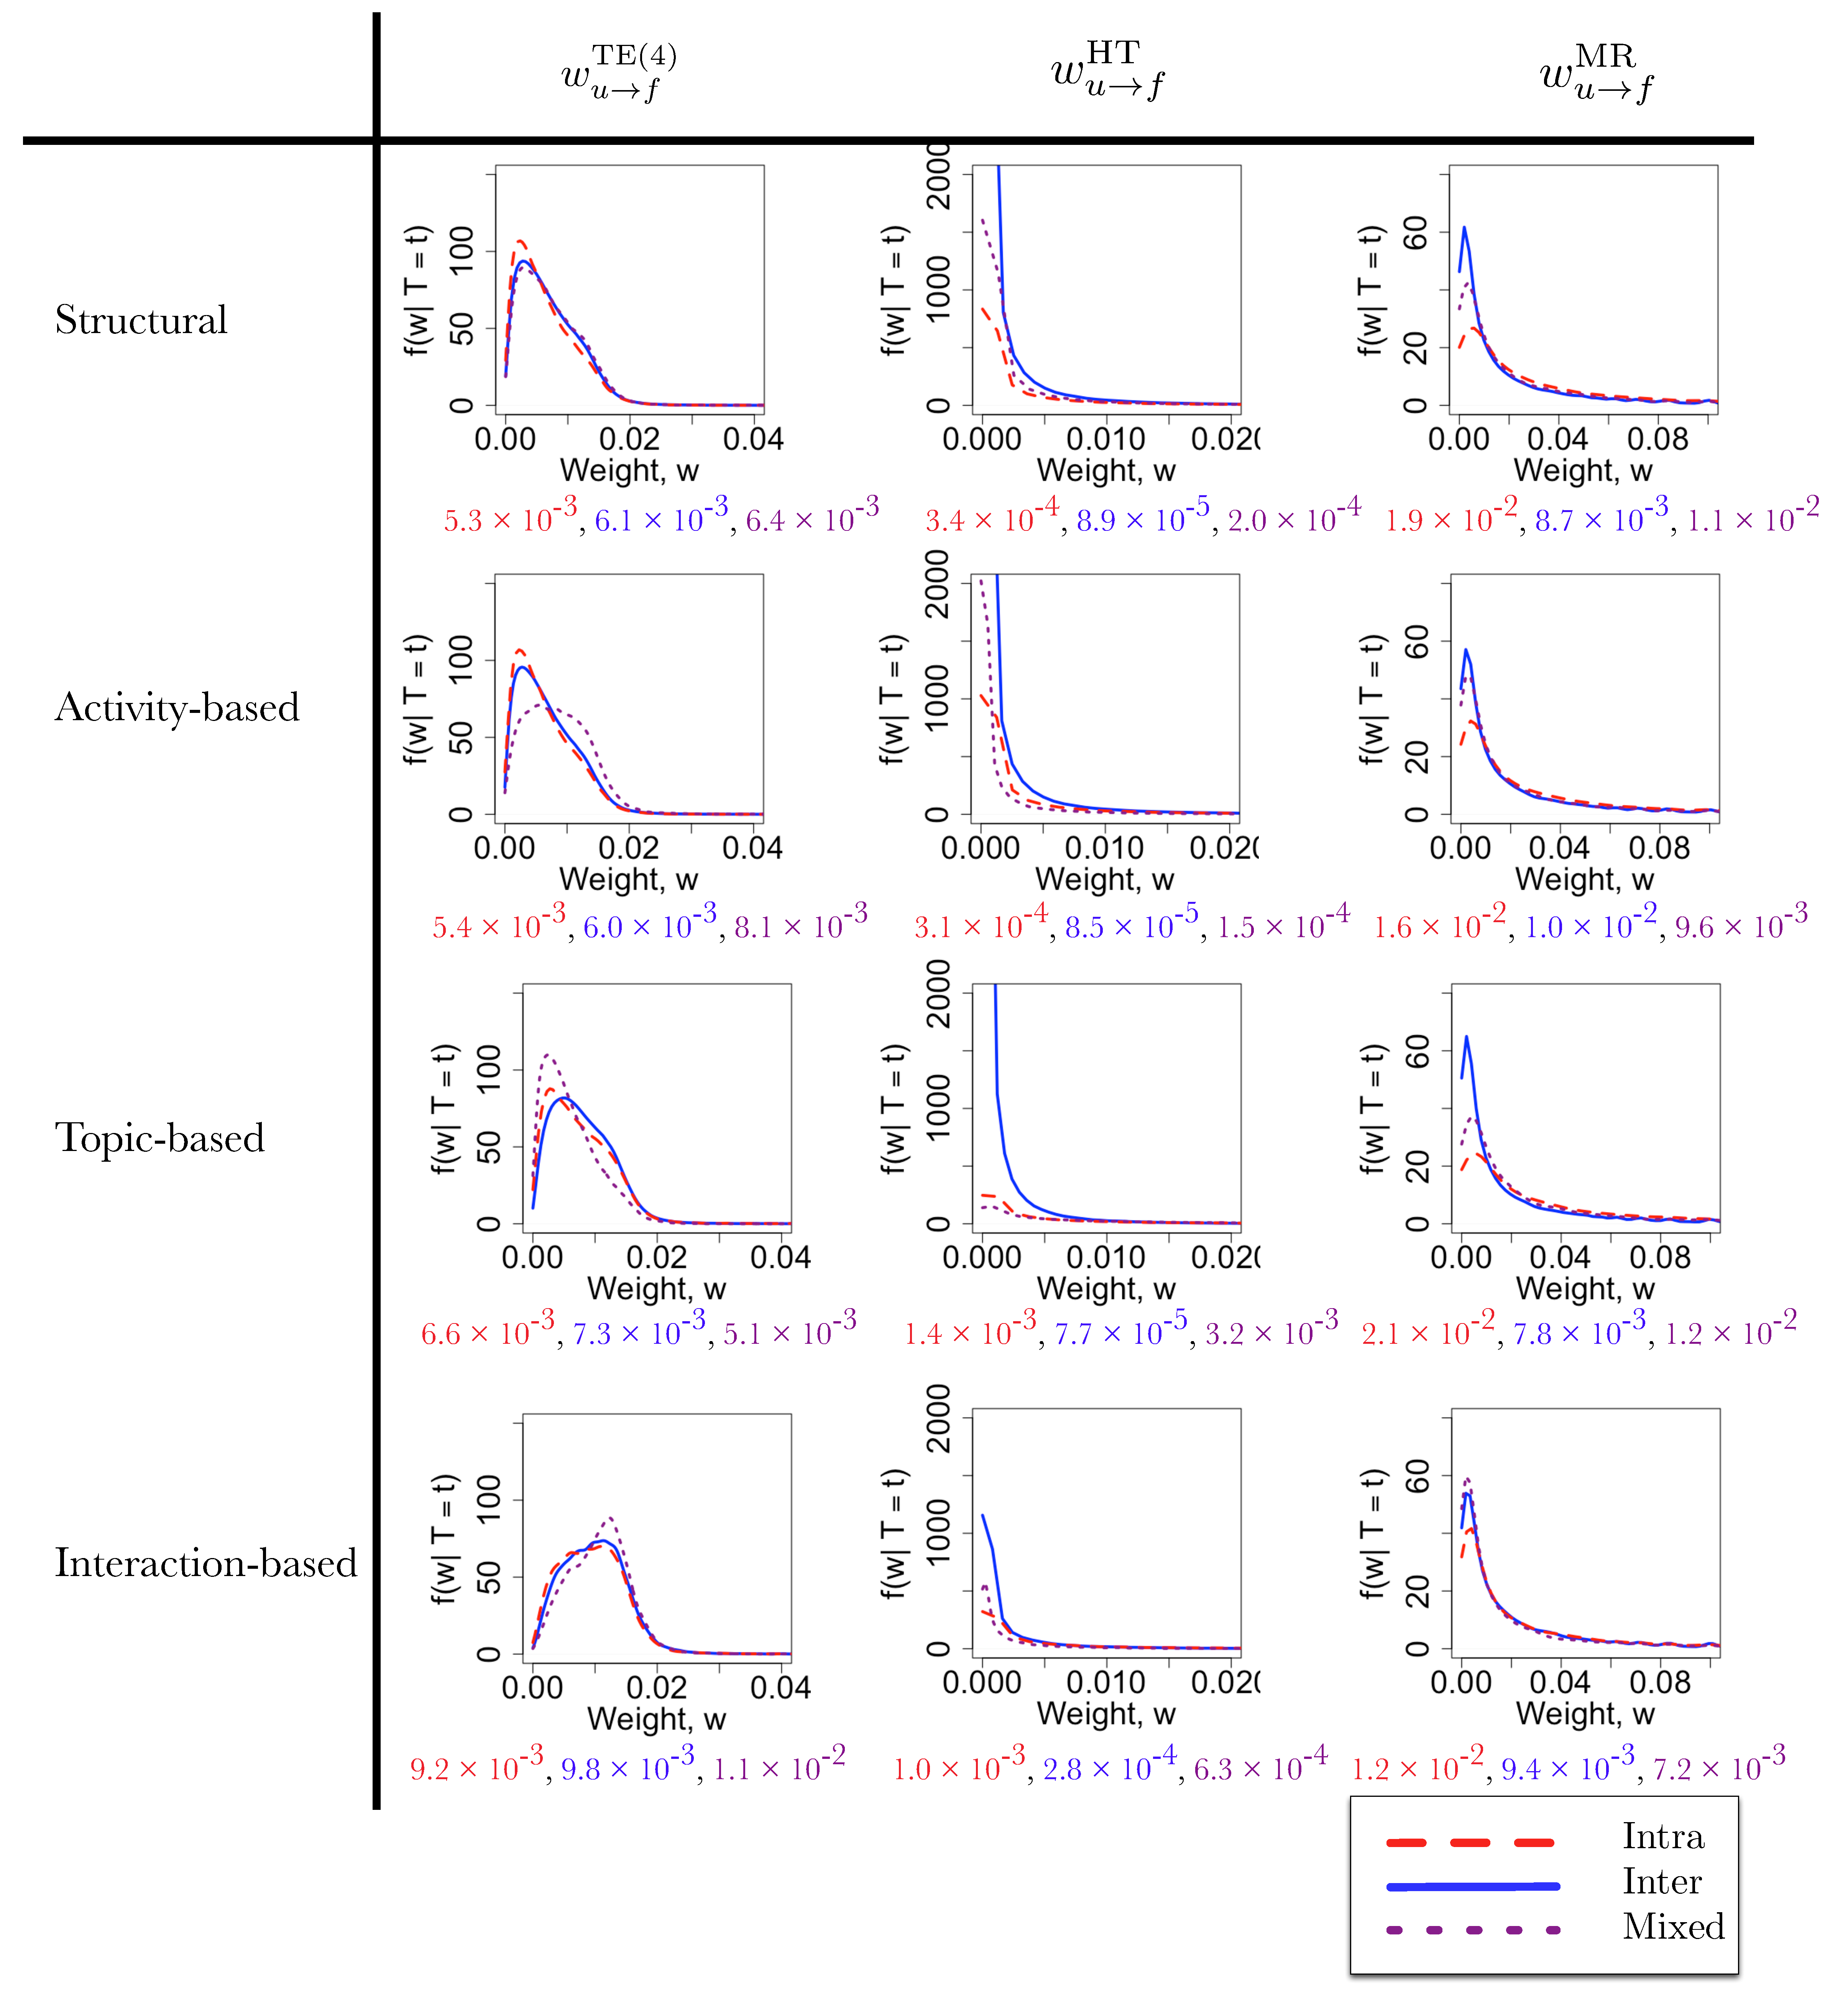
\includegraphics[width=1\textwidth]{densities-edges.eps}
	\caption{The density of edge weights for different community types (rows) and weight types (columns). The red,  blue, and magenta values below each collection of densities indicate the median of weight on intra-, inter-, and mixed-edges, respectively.}
	\label{Fig-distributions_by_types}
\end{figure}